In this chapter we describe the system, which has been used for the generation of CS, the governing equations,  and the methodology to solve and analyze the governing equation. 
\section{System}
We have used broad-area semiconductor laser cavity comprised of a Vertical-Cavity Sur-
face Emitting Laser (VCSEL) with a saturable absorber (SA) and coupled to a frequency-
selective feedback element(FSF) to study the formation of CS \cite{hachairCavitySolitonsBroad2004}. VCSELs are a class of semiconductor lasers characterized by their vertical emission\
relative to the surface of the semiconductor substrate. They offer several advantages over\
traditional edge-emitting lasers, including lower threshold currents, circular beam profiles,\ 
and the ability to be fabricated in dense two-dimensional arrays. When integrated with a saturable absorber,\
the VCSEL can exhibit a range of nonlinear dynamical behaviors, crucial for the formation of cavity solitons.

A saturable absorber is a material whose absorption decreases with increasing light intensity.\
This nonlinearity is essential for the self-organization processes leading to soliton formation. In the context\
of VCSELs, the saturable absorber enables the laser to support super-stable localized cavity solitons that can persist indefinitely under constant pumping conditions.

The addition of a frequency-selective feedback element further refines the system. The FSF element selectively\
reflects specific frequencies back into the laser cavity, effectively narrowing the emission spectrum and enhancing the stability of the cavity solitons. This selective\
feedback can be implemented using various optical components, such as Bragg gratings or Fabry-Pérot interferometers.

The dynamics of this complex system are often modeled by the Complex Ginzburg-Landau Equation (CGLE) \cite{chatePhaseDiagramTwodimensional1996,ComplexGinzburgLandauEquation,mayteevarunyooOneTwodimensionalModes2018}. \
The CGLE is a partial differential equation that describes the evolution of a complex field envelope and encompasses key physical processes such\
as dispersion, nonlinearity, gain, and loss. In the context of VCSELs with a saturable absorber and FSF \cite{bacheCavitySolitonLaser2005a,firthCavitySolitonProperties2009}, 
the CGLE captures the interplay between diffraction, nonlinearity, and feedback, which governs the formation and stability of cavity solitons \cite{nagiBroadbandCavitySoliton2022,kaurGenerationDynamicsOne2017a}.

The general form of the CGLE used in this context is:
\begin{equation}
    \frac{\partial E}{\partial t} = E + (1 + i\alpha)\nabla^2 E - (1 + i\beta)|E|^2E + \gamma E    
\end{equation}



where \(E\) is the complex field envelope, \(\alpha\) and \(\beta\) are real coefficients representing the linear and nonlinear contributions to the refractive index, respectively, and \(\gamma\) represents the gain/loss term modulated by the saturable absorber and the feedback.

The theoretical framework provided by the CGLE has been instrumental in predicting and explaining the rich variety of dynamical behaviors observed in experiments, including the formation, interaction, and stability of cavity solitons. The solitonic solutions of the CGLE, known as dissipative solitons, are particularly relevant for optical systems where gain and loss are inherently present.
This configuration has garnered considerable attention due to its potential applications in optical communication and information processing.
% ### References

% 1. Agrawal, G. P., & Dutta, N. K. (1993). Long-wavelength Semiconductor Lasers. Van Nostrand Reinhold.
% 2. Barland, S., et al. (2002). Cavity solitons as pixels in semiconductor microcavities. *Nature*, 419(6908), 699-702. [DOI: 10.1038/nature01049](https://doi.org/10.1038/nature01049)
% 3. Genevet, P., et al. (2008). Cavity soliton laser based on mutually coupled semiconductor microresonators. *Physical Review Letters*, 101(12), 123905. [DOI: 10.1103/PhysRevLett.101.123905](https://doi.org/10.1103/PhysRevLett.101.123905)
% 4. Tanguy, Y., et al. (2008). VCSEL with optical feedback: Towards a controllable system for the study of dissipative solitons. *Physical Review Letters*, 100(1), 013907. [DOI: 10.1103/PhysRevLett.100.013907](https://doi.org/10.1103/PhysRevLett.100.013907)
% 5. Elsass, T., et al. (2010). Control of cavity solitons and dynamical states in a monolithic vertical cavity laser with saturable absorber. *The European Physical Journal D*, 59(1), 91-96. [DOI: 10.1140/epjd/e2010-00144-3](https://doi.org/10.1140/epjd/e2010-00144-3)
% 6. Brambilla, M., et al. (2011). Theoretical and experimental analysis of the interaction of cavity solitons in VCSELs with saturable absorber. *Physical Review A*, 83(3), 033835. [DOI: 10.1103/PhysRevA.83.033835](https://doi.org/10.1103/PhysRevA.83.033835)


\begin{figure}[h]
    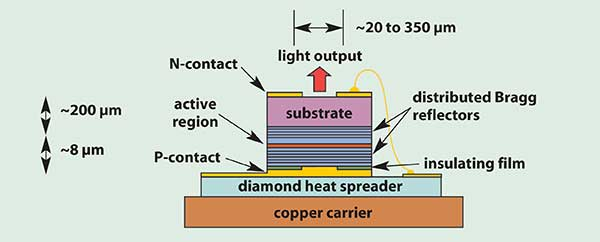
\includegraphics[scale=0.5]{VCSEL.jpg}
\end{figure}

\section{Mathematical modeling}
The cavity lasers, as described above can be modeled by, 2D CGLE which is given as below (\ref{CGLE evol eqn}).
\begin{eqnarray}
    &&\iota\frac{\partial E}{\partial t} + \left[\theta - \frac{\mu \alpha}{1+g_1|E|^2} + \frac{\gamma\beta}{1+sg_2|E|^2} + \Delta \right]E - bE	+V(x,y)E \cr
    &&= \iota\left[-1 + \frac{\mu}{1+g_1|E|^2} - \frac{\gamma}{1+sg_2|E|^2}+\alpha_{ns}+a\right]E \\
    && \cr
    && \frac{\partial E}{\partial t} = \left[-(1- i \theta) + \frac{\mu(1-\iota \alpha)}{1+g_1|E|^2} - \frac{\gamma(1-\iota\beta)}{1+sg_2|E|^2} +\alpha_{ns} + a + - i b +i\Delta\right] E + iV(x,y) E \cr
    && \label{CGLE evol eqn}
\end{eqnarray}
Where $a$ and $b$ are given as follows:

\begin{eqnarray}
&& a = \left(\frac{\sigma\lambda^2}{(\lambda^2+\omega^2)}\right) \cr
&& b = \left(\frac{\sigma\lambda\omega}{(\lambda^2+\omega^2)}\right)  \nonumber 
\end{eqnarray}
and the the different parameters used to model VCSEL are:
$\theta$ detuning parameter ;
$\mu$ : pumping parameter for active medium ;
$\alpha$ : Linewidth Factor for active medium ;
$g_1 , g_2$: coefficients of saturation of active and passive media respectively. ;
$s$: saturation parameter ;
$\beta$: linewidth factor for passive medium ;
$\gamma$: pumping parameter for passive medium ;
$\alpha_{ans}$: non-saturable loss ;
$\lambda$: bandwidth ;
$\sigma$: Feedback-strength ;
$\omega$: Resonance Frequency ;
$(a+ib)$: represents the feedback field ;
$V(x,y)$: is the spatially varying potential function .

The values for the above parameters for which the soliton solutions can exist, can be found analytically using Lagrangian Variational Method \cite{kaurGenerationDynamicsOne2017a,kaurCavitySolitonMolecules2018}\
for simple system without the potential. The analytical approach is limited to very simple systems. As the system becomes complex,\
it becomes extremely difficult to solve analytically. 


\section{Approach}
    Analytically solutions to PDEs is extremely limited to special and simple cases. It is more parsimonious to use different approximate methods to\
get understanding of the nature of PDE in question. Amongst many different numerical methods, Split Step Fourier method is one popular choice for its reasonable demands of computational resources. This method is\
used in various senarios such as in light pulse propagation in optical fibers, dynamics of optical microresonator, and finding soliton solutions.

    
Split-step Fourier method (SSFM) is based on seperating the linear and nonlinear part of the equations and dealing with them seperately in small steps. Linear part is dealt in frequency domain by Fourier\
tranforming it, while nonlinearity is dealt in time domain.

\subsection{Split-step Fourier Method (SSFM)}
Split-step Fourier Method (SSFM) is an effective and powerful numerical technique for solving partial differential equations (PDEs) which have linear\
and non-linear terms and can be separated into them \cite{agrawalNonlinearFiberOptics2001,ablowitzInverseScatteringTransformFourier1974}. This method combines the advantages of Fourier transforms for handling spatial derivatives and\
explicit time-stepping schemes for nonlinear terms. The method involves splitting the equation into linear and nonlinear parts and solving each part\ 
sequentially within a small time step $\Delta t$. In the present case, with CGLE, we can split it into dispersion terms and non-linear terms as in (\ref{diffraction operator}) and (\ref{nonlinearity operator})\
and then proceed with the steps as described below.

\begin{eqnarray}
    && \mathbf{D} = \left(-1 + i\theta + a -ib - iK_x^2 -iK_y^2\right) \frac{h}{2} \label{diffraction operator}\\
    && \mathbf{N} = \left(iV(x,y)+ \frac{\mu (1-i\alpha)}{1+g_1|E|^2}- \frac{\gamma (1-i\beta)}{1+s g_2|E|^2} + \alpha_{ns}\right)h \label{nonlinearity operator}
\end{eqnarray}
where h is the step size.

In the SSFM, we approximate the solution over a time step $\Delta t$ by first solving the linear part in the Fourier domain, then solving the nonlinear part in the spatial domain.\
The Split-Step Fourier method for solving the CGLE involves the following steps:

\begin{enumerate}
  \item \textbf{Initialization}: Start with the initial condition $u(x, y, 0)$.
  
  \item \textbf{Fourier Transform}: Convert the spatial domain field $u(x, y, t)$ to the Fourier domain using the Fast Fourier Transform (FFT):
  \begin{equation}
      \hat{u}(k_x, k_y, t) = \mathcal{F}\{u(x, y, t)\},
  \end{equation}
  where $k_x$ and $k_y$ are the wave numbers in the x and y directions, respectively.  

  \item \textbf{Linear Evolution}: Solve the linear part in the Fourier domain:
  \begin{equation}
      \hat{u}(k_x, k_y, t + \Delta t) = \hat{u}(k_x, k_y, t) \exp\left\{(1 + i\alpha)k^2 \Delta t\right\},
  \end{equation}
  where $k^2 = k_x^2 + k_y^2$.

  \item \textbf{Inverse Fourier Transform:} Convert the field back to the spatial domain:
  \begin{equation}
      u(x, y, t + \Delta t/2) = \mathcal{F}^{-1}\{\hat{u}(k_x, k_y, t + \Delta t)\}.
  \end{equation}

  \item \textbf{Nonlinear Evolution}: Solve the nonlinear part in the spatial domain:
  \begin{equation}
      u(x, y, t + \Delta t) = u(x, y, t + \Delta t/2) \exp\left\{(1 - (1 + i\beta)|u(x, y, t + \Delta t/2)|^2) \Delta t\right\}.
  \end{equation}

  \item \textbf{Repeat}: Iterate the process over multiple time steps until the desired time $T$ is reached.

\end{enumerate}


This method efficiently separates the linear and nonlinear components of the CGLE, allowing for stable and accurate numerical solutions. It is widely\
used in computational physics and nonlinear optics for studying pattern formation, wave propagation, and turbulence.
\subsubsection{Advantages and Applications}
The SSFM is particularly advantageous due to its efficiency and accuracy in handling both dispersion and nonlinearity in wave equations. It is widely\
used in the study of optical solitons, wave propagation in nonlinear media, and various other fields where the CGLE plays a pivotal role \cite{wangEfficientSplitstepCompact2013, goldmanNovelMethodSimulating1995,agrawalNonlinearFiberOptics2001}.

The method's ability to decouple the linear and nonlinear components allows for larger time steps than would be feasible with traditional finite-difference methods,\
making it a powerful tool in computational physics and applied mathematics.

